\subsection{Distancesensor}

\begin{figure}[ht]
	\centering
	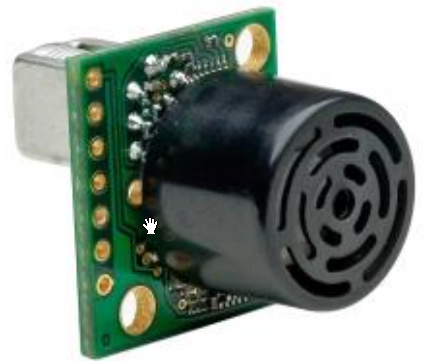
\includegraphics[scale=0.4]{../fig/billeder/distancesensor.png}
	\caption{Distancesensor MaxSonar1202}
	\label{fig:ds_pic}
\end{figure}

Distancesensorerne er tilføjet systemet for at kunne videregive data til AKS-klassen så denne kan tage de nødvendige forholdsregler. 
Det er valgt at benytte ultralydssensorer af type MaxSonar1202-typen \cite{lib:maxsonar} til formålet. 
Disse levede op til de stillede krav til systemet om rækkevidde, interface og kommunikationsprotokol.
På sensorprintet var der ydermere mulighed for at tilgå status-pin og alt.-adresse pin. Dette blev dog ikke benytte i projektet og der er derfor ikke gjort brug af disse features.

De fire sensorer er montering parvis for og bag på bilen, på figur \ref{fig:ds_mont} ses sensorerne ''Front Left'' og ''Front Right''. 

\begin{figure}[ht]
	\centering
	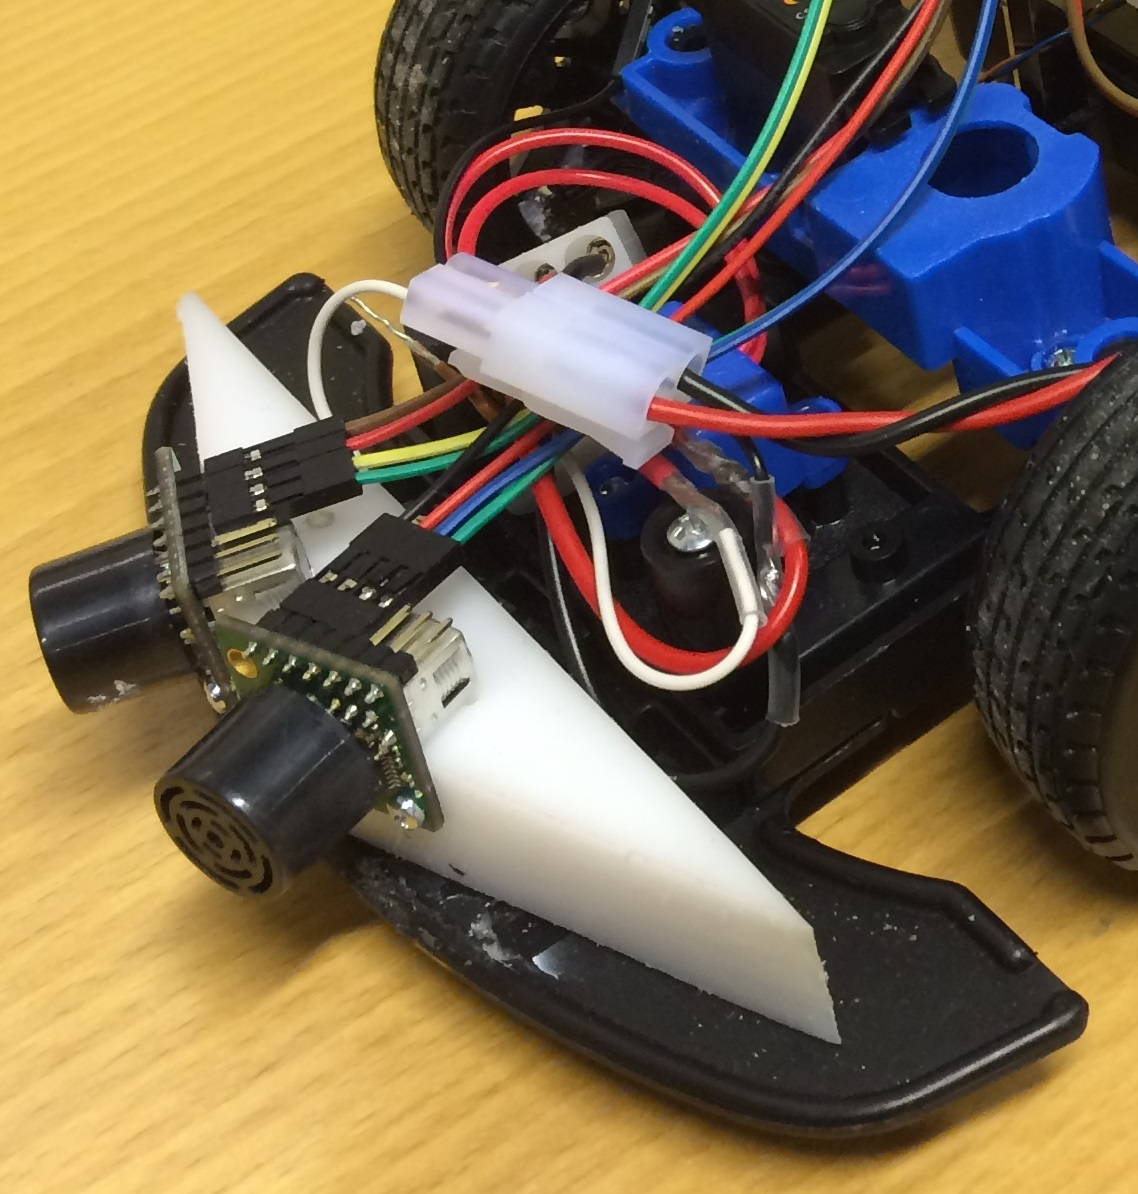
\includegraphics[scale=0.1]{../fig/billeder/distancesensor_montering.jpg}
	\caption{Distancesensorer monteret på fronten af AU2}
	\label{fig:ds_mont}
\end{figure}

De fire sensorer sidder på fælles \IIC bus med pull-up resistor på datalinjen (\texttt{SDA}) og clocken (\texttt{SCL}). Denne del af bussen har PSoC'en som Master og sensorerne som slaver. 

